\chapter{Introduction}
\pagenumbering{arabic}\hspace{3mm}

Image processing libraries these days (eg. Open CV) uses the conventional methods which have the possibility to be outperformed by methods which leverage the power of artificial intelligence. Some recent research have shown that some of these AI based methods are able to perform atleast as good as conventional approaches. The aim of this project is to implement, apply and possibly improve upon the existing approaches in Digital Image Processing and Computer Vision. These common tasks can include (not limited to) applications like: Image Compression, Denoising, Super Resolution, Flow Estimation, Object Detection, etc.


\section{Image Processing}

\begin{figure}[!ht]
    \centering
    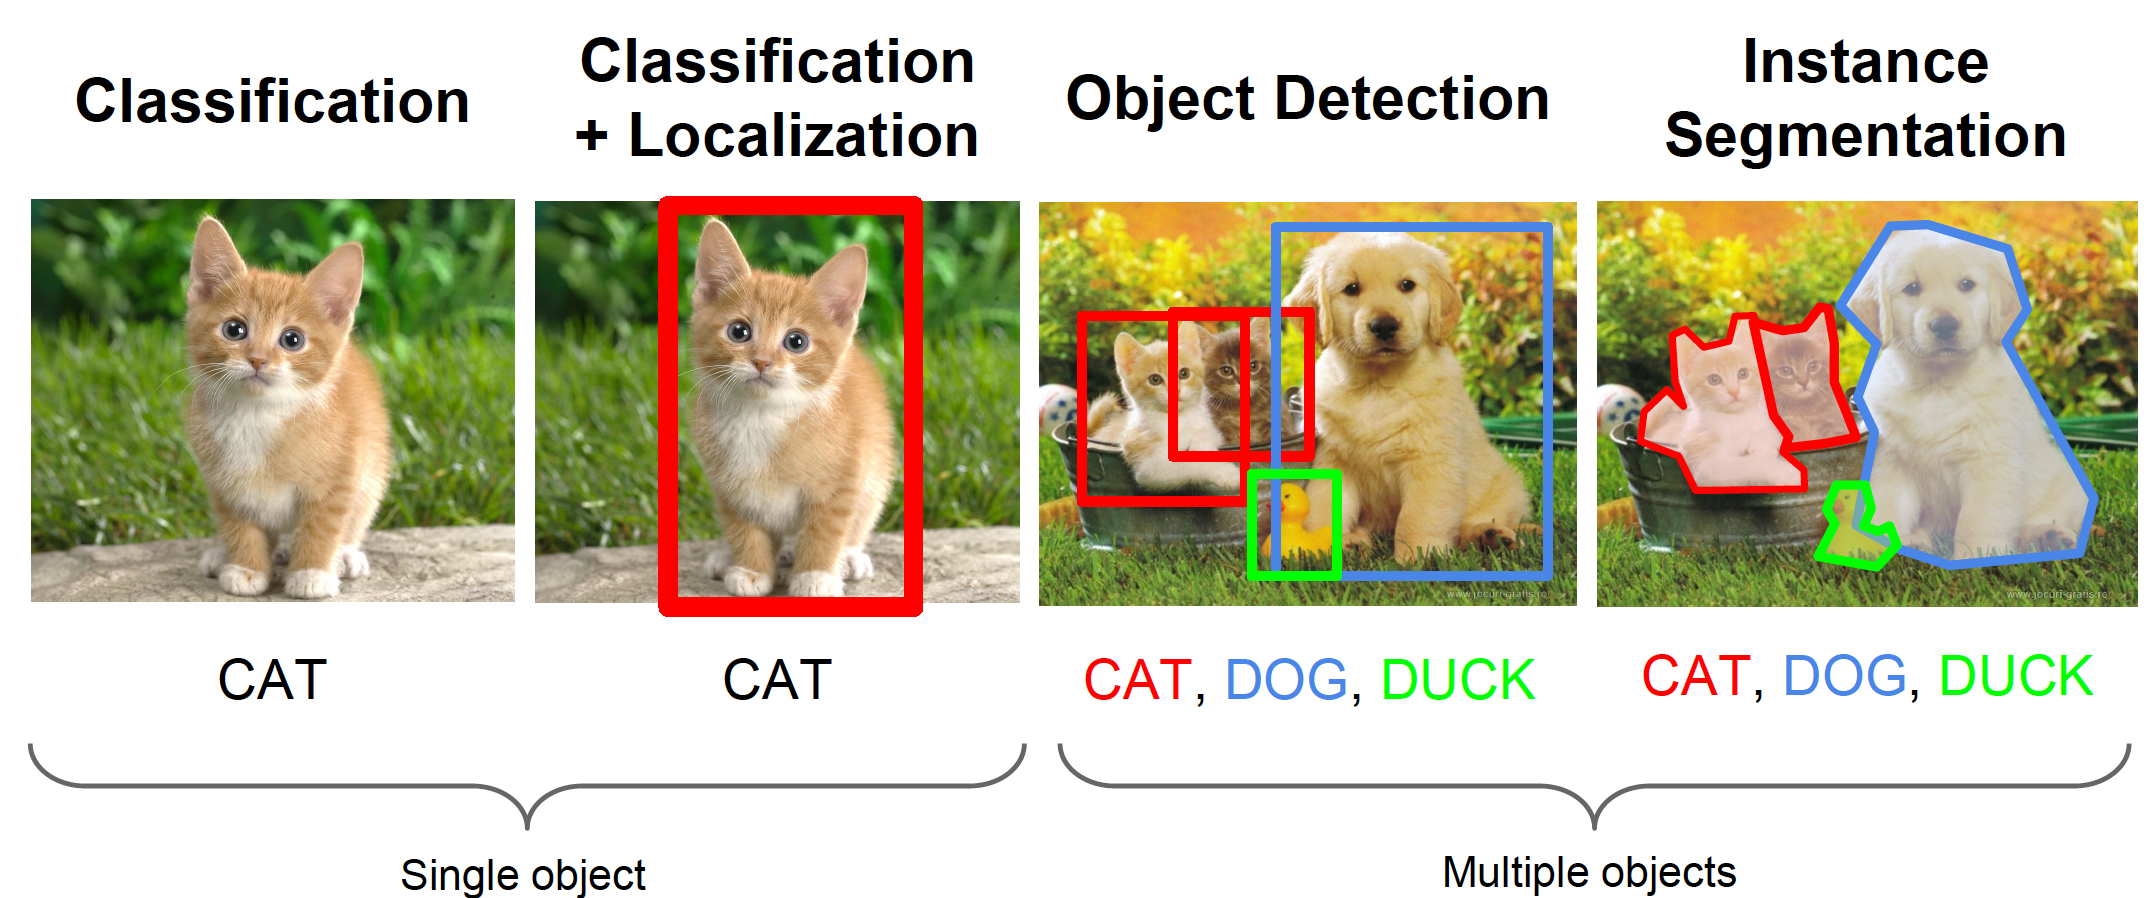
\includegraphics[width=0.75\textwidth]{fig/1-1.png}
    \captionsource{Examples of pattern recognition}
    {\href{https://www.cs.cornell.edu/courses/cs4670/2016sp/lectures/lec41_recowrapup_web.pdf}{www.cs.cornell.edu}}
    \label{fig:exPatternRecognition}
\end{figure}

Image processing is manipulating an image in order to enhance it or extract information from it. It is widely useed in medical visualization, biometrics, self-driving vehicles, gaming, surveillance, and law enforcement. It can used in various ways: visualization, restoration, imformation retrieval, pattern recognition, etc.

General approach of image processing involves eight key phases: image acquisition, image enhancement, image restoration, color space transformation, compression or decompression, morphological processing, recognition, and representation. It is very difficult to carry out these steps manually on a very big data, this is where AI and ML algorithms become very helpful.

\begin{figure}[!ht]
    \centering
    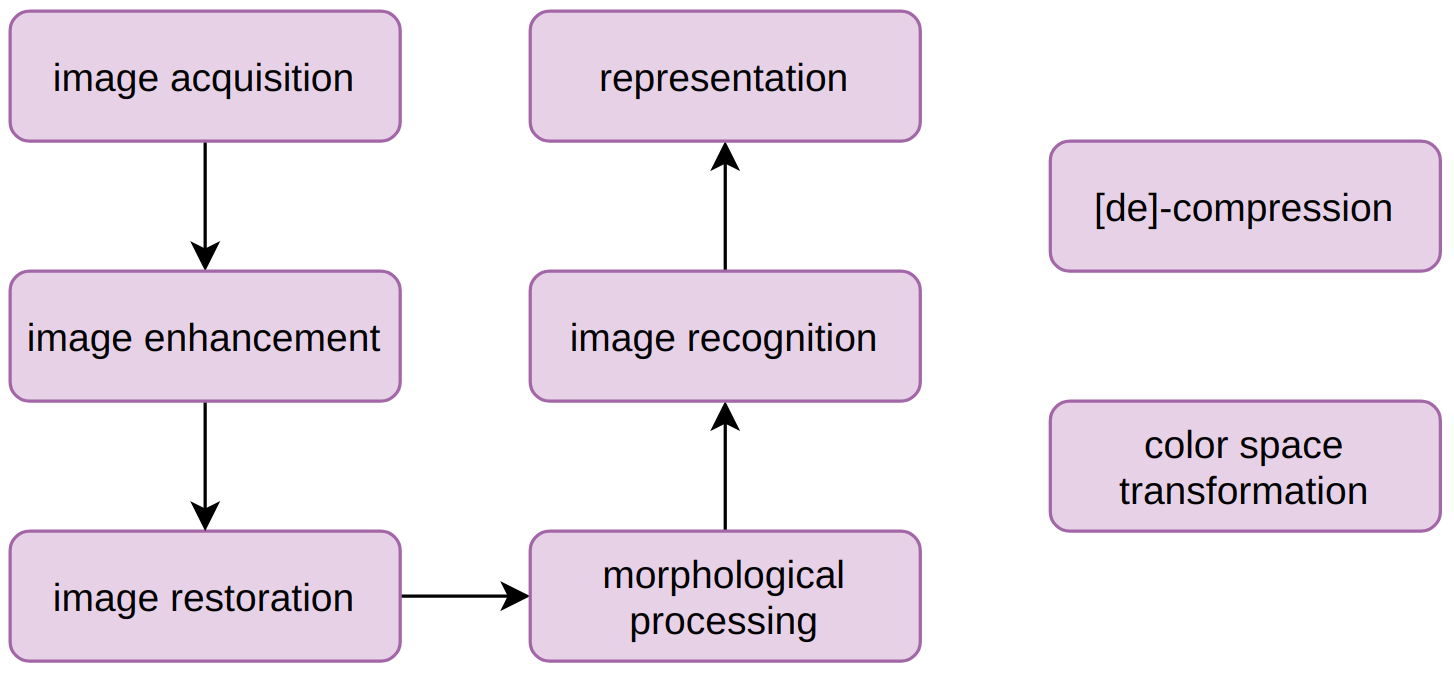
\includegraphics[width=0.75\textwidth]{fig/1-2.png}
    \caption{Key phases of image processing}
    \label{fig:keyPhasesOfImageProcessing}
\end{figure}

\section{2nd Section name}

2nd Section

\section{Organization of The Report}

You can write the about organization of your report in the following manner.

This chapter provides a background for the topics covered in this
report. We provided a description of wireless ad hoc networks, and
their applications. Then we described the network model that
represents the topology of wireless ad hoc networks \cite{Omar2016}. In this
chapter it is shown that the virtual backbone for wireless ad hoc
networks can be represented by a connected dominating set. We
explained clustering concepts and lastly the difference between
centralized and distributed algorithms are also discussed. The
rest of the chapters are organised as follows: next chapter we
provide review of prior works. In Chapter 3 and 4, we discuss our
new algorithms for constructing small backbones for ad-hoc
wireless network. And finally in chapter 6, we conclude with some
future works.

